\subsection{Particle A}
Particle A is approximately \unit[24]{$\mu m$} long so it has a $\lambda$ close to 8 and the closest match for the asymmetry is $\epsilon = 0.02$. 

Using the algorithm described in section \ref{sec:matchorbit} we match the data from measurement 1 and 2 for particle A to find the closest matching $\epsilon$ and the best matching orbits. This is shown in Figure \ref{fig:particleAOrbitFit}. We can see that particle A is in a quasi-periodic sign changing orbit during measurement 1, it is matched to the lines indicating A B and C for the first, second and third stretches respectively.  After being shifted by the optical tweezers, particle A followed a periodic orbit during measurement 2. Measurement 2 is matched to the orbits D, E, F and G for the first, second, third and fourth stretches respectively. The stretches that do not have winding numbers listed in the figures had orbits that did not have enough variation in $n_z$ peaks to try to estimate a winding number. 

Note that the orbits shown in Figures \ref{fig:particleAOrbitFit}, \ref{fig:October1Particle4runs2and2Orbits}, and \ref{fig:October1Particle4_runs3and5Orbits} are not the exact orbits matched. The measurements were matched to Poincaré maps with more orbits, but due to aliasing issues of printing such Poincaré maps more sparse Poincaré map are used. Each stretch is printed on the closest matching orbit for $\psi = 0$. The winding numbers are based on the more accurate fit and the better fits are available at \url{http://goo.gl/jgzSXe}. 

\begin{figure}[H]
\begin{center}
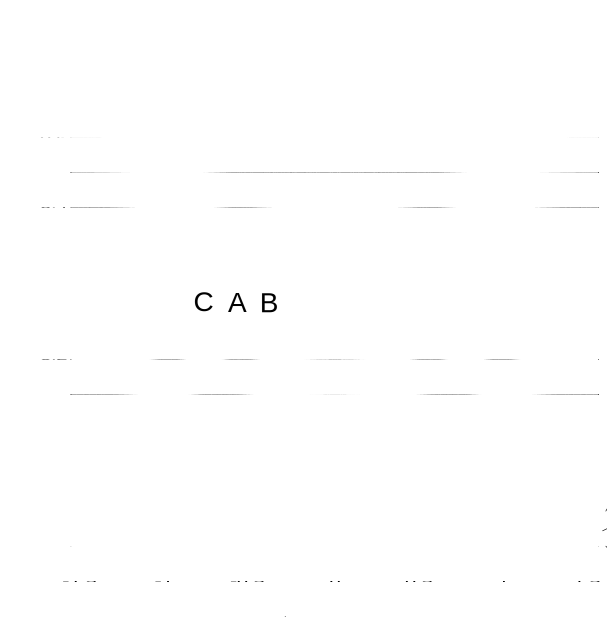
\includegraphics[width=\textwidth]{figures/results/orbitmatches/AmapAdded.pdf}
\end{center}
\caption{Black lines show the Poincaré map of the Jeffery's equations for $\lambda = 8$ and $\epsilon = 0.02$. The measured $\lambda$ was $8.2 \pm 0.1$. The orbits of the best fit theoretical fits to measurements are highlighted stretch by stretch. None of the orbits for this particle had any large variations despite being very close to $n_z=0$. The winding numbers are within 50\% of the estimates but both are too low, suggesting that the $\epsilon$ might be too low.}
\label{fig:particleAOrbitFit}
\end{figure}

\subsection{Particle B}

The same procedure is repeated for particle B using the data from measurement 1,2, 3 and 4. To make the graph less cluttered it is split into two figures, Figure \ref{fig:October1Particle4runs2and2Orbits} for measurement 1 and 2 and Figure \ref{fig:October1Particle4_runs3and5Orbits} for measurement 3 and 4.

In Figure \ref{fig:October1Particle4runs2and2Orbits} particle B during measurement 1 is matched to quasi-period orbits. During stretch 1 and 2 indicated by A and B it is matched to quasi-periodic sign preserving orbits. After unexplained behaviour during a reversal stretched 3 and 4 are matched to the same sign-changing orbit indicated by C and D. After being shifted using the optical tweezers, stretches 1 through 6 during measurement 2 are matched to the highly periodic orbits indicated by E, F, G, H, I, and J respectively. 


In Figure \ref{fig:October1Particle4_runs3and5Orbits} the closest matched orbits for particle B during measurement 3 and 4 are shown. During measurement 3 the quasi-periodic sign-preserving orbits indicated by A, B and C are the closest matches to stretches 1,2 and 3.  After being shifted by the optical tweezers particle B followed a sign changing quasi-periodic orbit during measurement 4. The best matching orbits for the first, second, third and fourth stretch of measurement 4 are matched to the orbits indicated by D, E, F, and G respectively. 


\begin{figure}[H]
\centering
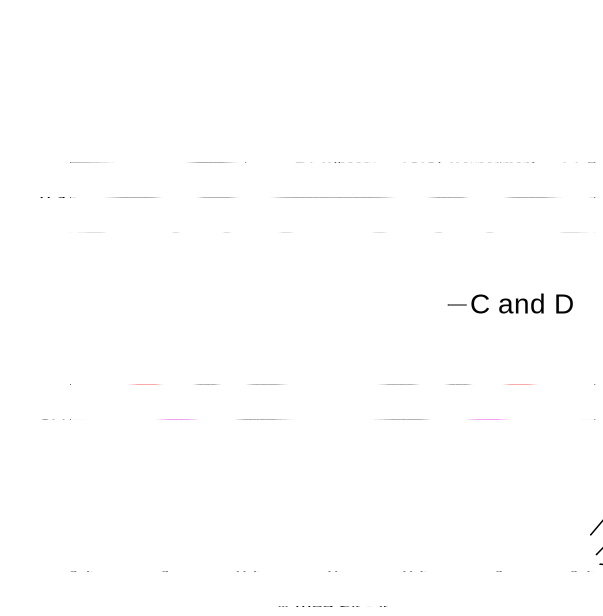
\includegraphics[width=\textwidth]{figures/results/orbitmatches/Bmap1Added.pdf}
\caption{Black lines show the Poincaré map of the Jeffery's equations for $\lambda = 7$ and $\epsilon=0.04$, the estimate of $\lambda$ from measurement was $6.7 \pm 0.1$. The highlighted orbits are the best fits to the stretches from measurements 1 and 2 of particle B. A-D are from measurement 1 and E-I from measurement 2.}
\label{fig:October1Particle4runs2and2Orbits}
\end{figure}


\begin{figure}[H]
\centering
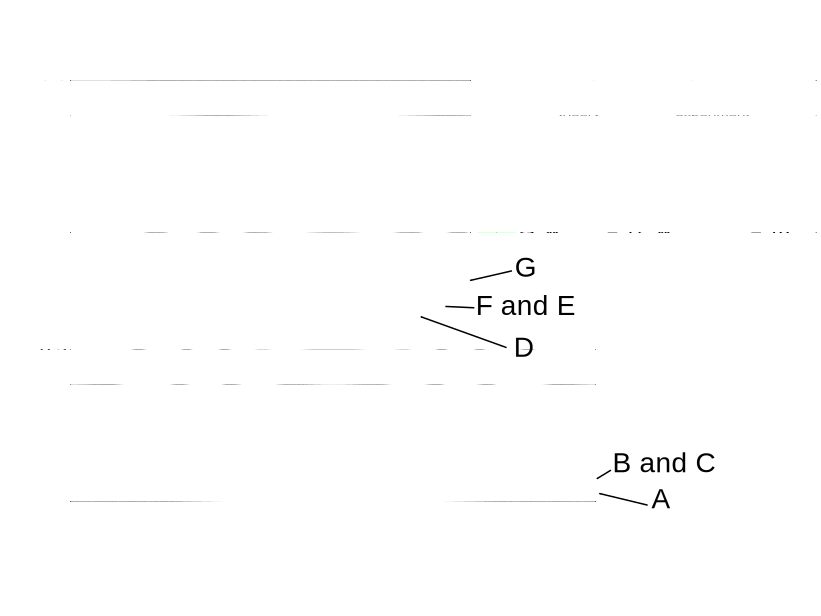
\includegraphics[width=\textwidth]{figures/results/orbitmatches/Bmap2Added.pdf}
\caption{Black lines show the Poincaré map of the Jeffery's equations for $\lambda = 7$ and $\epsilon = 0.04$. the estimate of $\lambda$ from measurement was $6.7 \pm 0.1$ . The highlighted orbits are the best fits to the stretches from measurements 3 and 4 of particle B. A-C are from measurement 3, and D-G from measurement 4.}
\label{fig:October1Particle4_runs3and5Orbits}
\end{figure}


